\newcommand{\bydef}{\overset{\scriptscriptstyle\Delta}{=}}
\newcommand{\EE}{\mathbb{E}}
\newcommand{\PP}{\mathbb{P}}
\begin{abstract}

\end{abstract}

\section{Introduction}

\section{Problem statement and modelling}
We aim to build an agent that solves an empty  $6\times6$ grid world, e.g., reaching the green cell as illustrated in Figure \ref{fig:mini-grid}. The agent (red triangle) interacts with the environment through observations, actions and rewards. We use the \texttt{mini-grid} API from the Farama foundation to simulate the environment.
\begin{figure}[H]
	\centering
	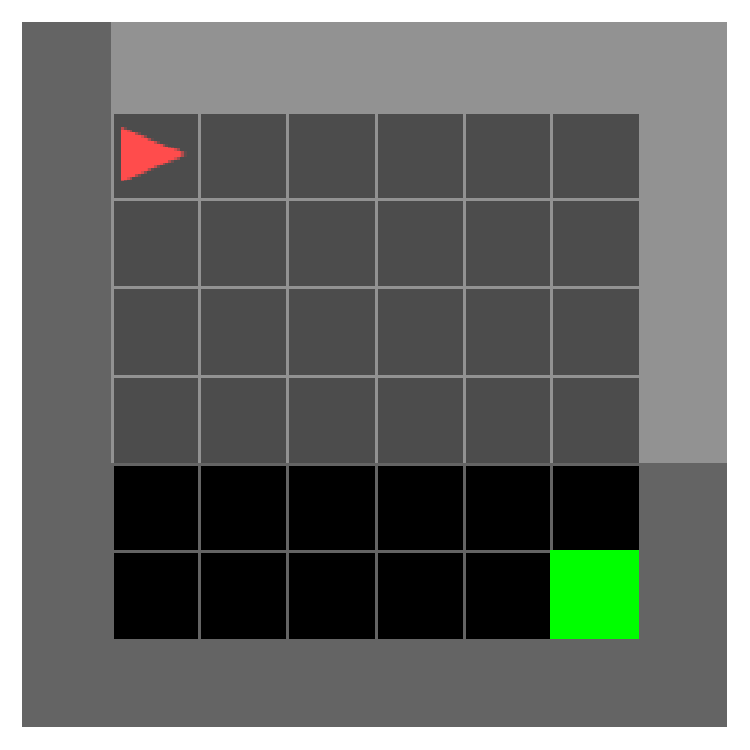
\includegraphics[width=0.9\linewidth]{figures/grid_world.pdf}
	\caption{The \texttt{MiniGrid-Empty-8x8-v0} environment}
	\label{fig:mini-grid}
\end{figure}

Depending on our configuration, the state can be a tensor or an image which is returned after each action. The agent has eight possible actions, but we only use three: turn left and right and move forward. In this setting, we deal with an episodic task, and for each episode, the agent can perform at most 256 steps.

If the agent reaches the target, it receives a reward $r$ defined by:
\begin{equation}
	r = 1 - 0.9\times \frac{\text{Number of steps}}{\text{Maximum number of steps}}
\end{equation}
otherwise, the reward is zero.


Therefore our task is to make the agent learn how to move in this grid in such a way that it maximizes its reward. For this particular environment, the agent can get at most a reward of $0.9613$ with $11$ steps. But for this work, we will consider $0.9578$ as the optimal reward corresponding to 12 steps.

\section{Reinforcement Learning technique}
In this era, reinforcement learning is widely used to solve the problem of programming intelligent agents that learn how to optimise a specific task such as playing a game, or autonomous vehicle. This is done by learning a policy for sequential decision problems that maximize the discounted  cumulative future reward:
\begin{equation}
	G_t \bydef \sum_{k=t+1}^{T} \gamma^{k-t-1}R_k
\end{equation}
Where $R$ is the reward, $\gamma\in [0,1]$ is the discount factor that controls the importance fro immediate reward (near to 0) or future reward (near to 1). The agent learns the optimal policy without being explicitly told if its actions are good or bad using the reinforcement learning model depicted in Figure \ref{fig:RL}.


\begin{figure}
	\centering
	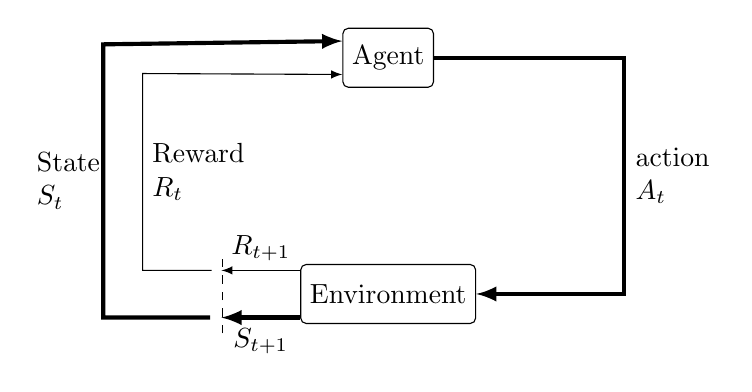
\begin{tikzpicture}
		\node[draw, rounded corners=2pt, minimum height=.75cm] (agent) at (0,0) {Agent};
		\node[draw, rounded corners=2pt, minimum height=.75cm] (env) at (0,-3) {Environment};
		\draw[->, >=latex,line width=1.5pt] (agent) -- (3, 0) -- node[right,midway, text width=1cm] {action\\$A_t$} (3, -3) -- (env);
		\draw[->, >=latex] (env.165) --node[above] {$R_{t+1}$} ++(-1, 0) node (r) {};
		\draw[->, >=latex, line width=1.5pt] (env.195) --node[below] {$S_{t+1}$} ++(-1, 0) node (s) {};
		\draw[->, >=latex] (r) -- ++(-1, 0) --node[right, midway, text width=1cm] {Reward\\$R_t$} ++(0, 2.5)-- (agent.200);
		\draw[->, >=latex,line width=1.5pt] (s)-- ++(-1.5, 0) --node[left=-0.3cm, midway, text width=1cm] {State\\$S_t$} ++(0, 3.47) -- (agent.160);
		\draw[dashed] (-2.1, -3.5)--(-2.1, -2.5);
	\end{tikzpicture}
	\caption{Reinforcement learning Model}
	\label{fig:RL}
\end{figure}

Several algorithms/techniques can be used  to solve our problem with reinforcement learning, in the next section we will look:
\begin{itemize}
	\item Q-Learning
	\item SARSA (State-Action-Reward-State-Action)
	\item Deep Q-Network
	\item Deep Q-Network with RGB Image techniques.
\end{itemize}
The algorithm \ref{algo:rl_skel} show the skeleton shared by these RL algorithms.
\begin{algorithm}
	Parameters:$\ldots$\\
	\ForEach{episode}{
		(Re)Initialize the environment\\
		\ForEach{step}{
			Act and consider the observation and reward\\
			\textbf{Steps specific to each methods}\\
			\If{done or truncated}{
				Some steps for metric and monitoring\\
			}
		}
	}
	\caption{RL Algorithm Skeleton}
	\label{algo:rl_skel}
\end{algorithm}
In addition to that, we also use the $\epsilon$-greedy strategy to select the action to be performed by the agent. The agent uniformly samples an action from the possible action for the given state with a probability $\epsilon$ and uses the optimal action for the given state with a probability $1-\epsilon$. In the first case, we say that the agent is exploring, and in the second case we say that the agent is exploiting.


For this work we will start with a higher value of $\epsilon$ to allow the agent to explore the environment, then we decrease it slowly until we reach a small value, this will be controlled by :
\begin{equation}
	\epsilon_t = \epsilon_{min} + \left(\epsilon_{max} - \epsilon_{min}\right) \exp\left\{-\frac{t}{\Delta}\right\}
\end{equation}
Where $\Delta$ is the decay rate, a higher value corresponds to a slow decrease, and a small value corresponds to a fast decrease.
\section{Tabular methods: Q-Learning and SARSA}
The tabular method refers to the creation of a table called Q-table, containing the value of $Q(S_t=s, A_t=a)$. This value indicates how good is acting $a$ on the state $s$.

For the two algorithms that we present in this section, the observation (a $7\times3\times3$ array) will be converted into a string to create an MD5 hash to represent the given state.
\subsection{SARSA}
The SARSA algorithm is an on-policy method, which means it iteratively refines a single policy, that also generates control action within the environments. The update rule is defined by:
\begin{equation}\label{eq:sarsa}
	Q(S_t, A_t)\leftarrow Q(S_t, A_t) + \alpha[R_{t+1} + \gamma(S_{t+1}, A_{t+1}) - Q(S_t, A_t)]
\end{equation}
From the equation \eqref{eq:sarsa}, we obtain the Algorithm \ref{algo:sarsa} for the SARSA learning.
\begin{algorithm}
	Parameters: Step size $\alpha\in]0,1]$, small $\epsilon>0$\\
	Initialize $Q(s,a)$ for all $s\in\mathcal{S}^{+}$ and $a\in\mathcal{A}(s)$ arbitrarily, except that $Q(terminal-state, \cdot)=0$\\
	\ForEach{episode}{
		Initialize $S$\\
		Choose $A$ from $S$ using policy derived from $Q$ ($\epsilon$-greedy)\\
		\ForEach{step until $S$ is a terminal  state}{
			Take the action $A$, observe $R$, $S'$\\
			Choose $A'$ from $S'$ using policy derived from $Q$ ($\epsilon$-greedy)\\
			$Q(S, A)\leftarrow Q(S, A)$\\
			\phantom{$Q(S, A)\leftarrow$}$ + \alpha[R_{t+1} + \gamma(S', A') - Q(S_t, A_t)]$\\
			$S\leftarrow S'$\\
			$A\leftarrow A'$
		}
	}
	\caption{SARSA: on-policy learners to estimate the optimal Q-table}
	\label{algo:sarsa}
\end{algorithm}

\subsection{Q-Learning}
In contrast to SARSA, the $Q$-Learning algorithm is an off-policy algorithm, which means we optimise the target policy using different policies. The update rule is given by
\begin{equation}\label{eq:qlr}
	Q(S_t, A_t)\leftarrow Q(S_t, A_t) + \alpha[R_{t+1} + \gamma\max_a (S_{t+1}, a) - Q(S_t, A_t)]
\end{equation}
Since we have the Algorithm \ref{algo:qlr} for $Q$-learning methods.
\begin{algorithm}
	Parameters: Step size $\alpha\in(0,1]$, small $\epsilon>0$\\
	Initialize $Q(s,a)$ for all $s\in\mathcal{S}^{+}$ and $a\in\mathcal{A}(s)$ arbitrarily, except that $Q(terminal-state, \cdot)=0$\\
	\ForEach{episode}{
		Initialize $S$\\
		Choose $A$ from $S$ using $\epsilon$-greedy\\
		\ForEach{step until $S$ is a terminal  state}{
			Take the action $A$, observe $R$, $S'$\\
			Choose $A'$ from $S'$ using $\epsilon$-greedy\\
			$Q(S_t, A_t)\leftarrow Q(S_t, A_t) + \alpha[R_{t+1} + \gamma\max_a (S_{t+1}, a) - Q(S_t, A_t)]$\\
			$S\leftarrow S'$\\
		}
	}
	\caption{Q-learning algorithm to estimate the optimal $Q$-table}
	\label{algo:qlr}
\end{algorithm}



These two methods are powerful in dealing with a few states and actions, but not very efficient for numerous states and actions. We can replace the table with a function approximator as we will see in the next section.



\section{Function approximation: Deep $Q$-network}
The idea of function approximation is to replace the value function with its approximation instead of using a look-up table. The function can take
\begin{itemize}
	\item the state and action as input, and $q(s,a)$ as output,
	\item or the state as input and $q(s,a)$ as output.
\end{itemize}
This is illustrated in the figure \ref{fig:fct-approx}.
\begin{figure}
	\centering
	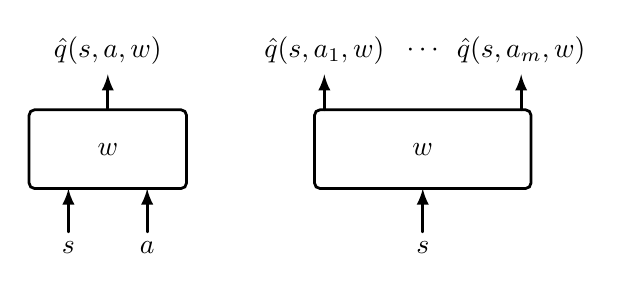
\begin{tikzpicture}
		\begin{scope}
			\node (s) at (-0.5,-1.25) {$s$};
			\node (a) at (0.5,-1.25) {$a$};
			\node (q) at (0,1.25) {$\hat{q}(s, a, \mbf{w})$};
			\node[draw, rounded corners=2pt, line width=1pt, minimum width=2cm, minimum height=1cm] (fct) at (0,0) {$\mbf{w}$};
			\draw[->, >=latex,line width=1pt, line cap=round] (s) --++(0,0.75);
			\draw[->, >=latex,line width=1pt, line cap=round] (a) --++(0,0.75);
			\draw[->, >=latex,line width=1pt, line cap=round] (fct) -- (q);
		\end{scope}
		\begin{scope}[xshift=4cm]
			\node (s) at (0,-1.25) {$s$};
			\node (q1) at (-1.25,1.25) {$\hat{q}(s, a_1, \mbf{w})$};
			\node (q2) at (0,1.25) {$\cdots$};
			\node (q3) at (1.25,1.25) {$\hat{q}(s, a_m, \mbf{w})$};
			\node[draw, rounded corners=2pt, line width=1pt, minimum width=2.75cm, minimum height=1cm] (fct) at (0,0) {$\mbf{w}$};
			\draw[->, >=latex,line width=1pt, line cap=round] (s) --++(0,0.75);
			\draw[<-, >=latex,line width=1pt, line cap=round] (q1) --++ (0, -.75);
			\draw[<-, >=latex,line width=1pt, line cap=round] (q3) --++ (0, -.75);
		\end{scope}
	\end{tikzpicture}
	\caption{Illustration of function approximation}
	\label{fig:fct-approx}
\end{figure}


In our case, we will use a neural network as a function approximation. Thus we will consider two types.

A feed-forward neural network (MLP) which takes a vector $\mbf{u}\in\RR^{49\times1}$ (state) as input and $q(s,a_1), q(s,a_2),q(s,a_3)$ as output.

Similarly, Convolutional Neural networks (CNN), take a stack of four frames (images) at four successive time steps, e.g. a $4\times56\times56$ tensor as input and the same output as the MLP, The architecture of these neural networks are described in respectively in REF-MLP and REF-CNN.


As we do not have any labels to train the networks, we use two networks: the \texttt{policy\_net} and \texttt{target\_net}. The first one is optimised with the \texttt{Adam} optimizer, while the second one is fixed, and used to generate a sort of label for the \texttt{policy\_net}. We also synchronize the weight of the two networks in a regular period of the training, to move toward the optimal values.


To train these networks, we need a dequeue (double end-queue) that stores a given number of the experience of the agent formed by the current state, action, next state, and reward, we call this a replay memory $\mathcal{D}$. As new experiences are added the oldest data is pushed out of the dequeue.
Once we reach have batch size (enough number) of experience, we start to sample from $\mathcal{D}$ and optimize the \text{policy\_net} parameter by minimizing the Mean Squared Error (MSE) given by:
\begin{equation}
	\mathcal{L} = \frac{1}{N}\sum{i=1}^{N}\left[R_i + \gamma\max_{a'}\hat{Q}(s_i', a', \mbf{w}^{-}) - \hat{Q}(s_i, a, \mbf{w})\right]^2
\end{equation}
where $R_i + \gamma\max_{a'}\hat{Q}(s_i', a', \mbf{w}^{-})$ is computed using \texttt{target\_net}, and $\hat{Q}(s_i', a', \mbf{w}^{-})$ is $0$ if $s_i'$ is terminal state, while $\hat{Q}(s_i, a, \mbf{w})$ is computed with \texttt{policy\_net}.


Note that, the input of these networks (observation) is normalized by rescaling their value between $[-1,1]$. In particular, we convert the RGB image into a grey-scale image for the CNN architecture.
We can summarize the whole process in the algorithm \ref{algo:dqn}.
\begin{algorithm}
	Initialize \texttt{policy\_net} and \texttt{target\_net}\\
	Initialize the environments\\
	Set the decay rate for the epsilon decreasing\\
	Set the updating period of \texttt{target\_net}\\
	Set the total step to $0$\\
	Create a replay memory $\mathcal{D}$\\
	\ForEach{episode}{
		Set step to 0\\
		Make a new episode\\
		Observe the first state\\
		\While{not( done or truncated)}{
			Choose $A$ from $S$ using policy derived from $Q$ ($\epsilon$-greedy)\\
			Increment the total training step\\
			Execute $A$, observe $R$ and the new state $S'$\\
			Store Transition $<S, A, S', R>$ in $\mathcal{D}$\\
			Compute the $\mathcal{L}$ and do a gradient descent step\\
			\If{updating period}{
				Copy the \texttt{policy\_net} parameter to \texttt{target\_net}
			}
		}
	}
	\caption{Training a DQN to estimate the optimal policy}
	\label{algo:dqn}
\end{algorithm}
\section{Hyper-parameters tuning and Evaluation}
\subsection{Hyper-parameters}
like all machine learning problems we have several parameters to tune to get the optimal results. Grid search is one of the best methods, it iterates through all the possible combinations of predefined parameters set. The drawback of this method is the time complexity which can explode considerably when we hyper-parameter space is big and the algorithm is quite slow.

So, instead of using that approach, we will use trial and error to find good hyper-parameters such as $\gamma$, $\alpha$, and the number of episodes. To do that we start we some values, and we adjust these parameters according to the obtained results.

\subsection{Model evaluation}
To evaluate the model, we run the agents in the environment for $1000$ episodes, then compute the completion rate, the reward average, and the averaged steps for each method.

We also investigate these values for the training process to assess the speed and efficiency of each method, in addition to the plot of the loss and accumulated rewards.
\section{Results and discussion}
In this section we discus about our results an present them. The smoothed plot were smoothed using the exponential moving average wit a factor of $0.7$.
\subsection{Q-Learning}
\begin{figure}[H]
	\centering
	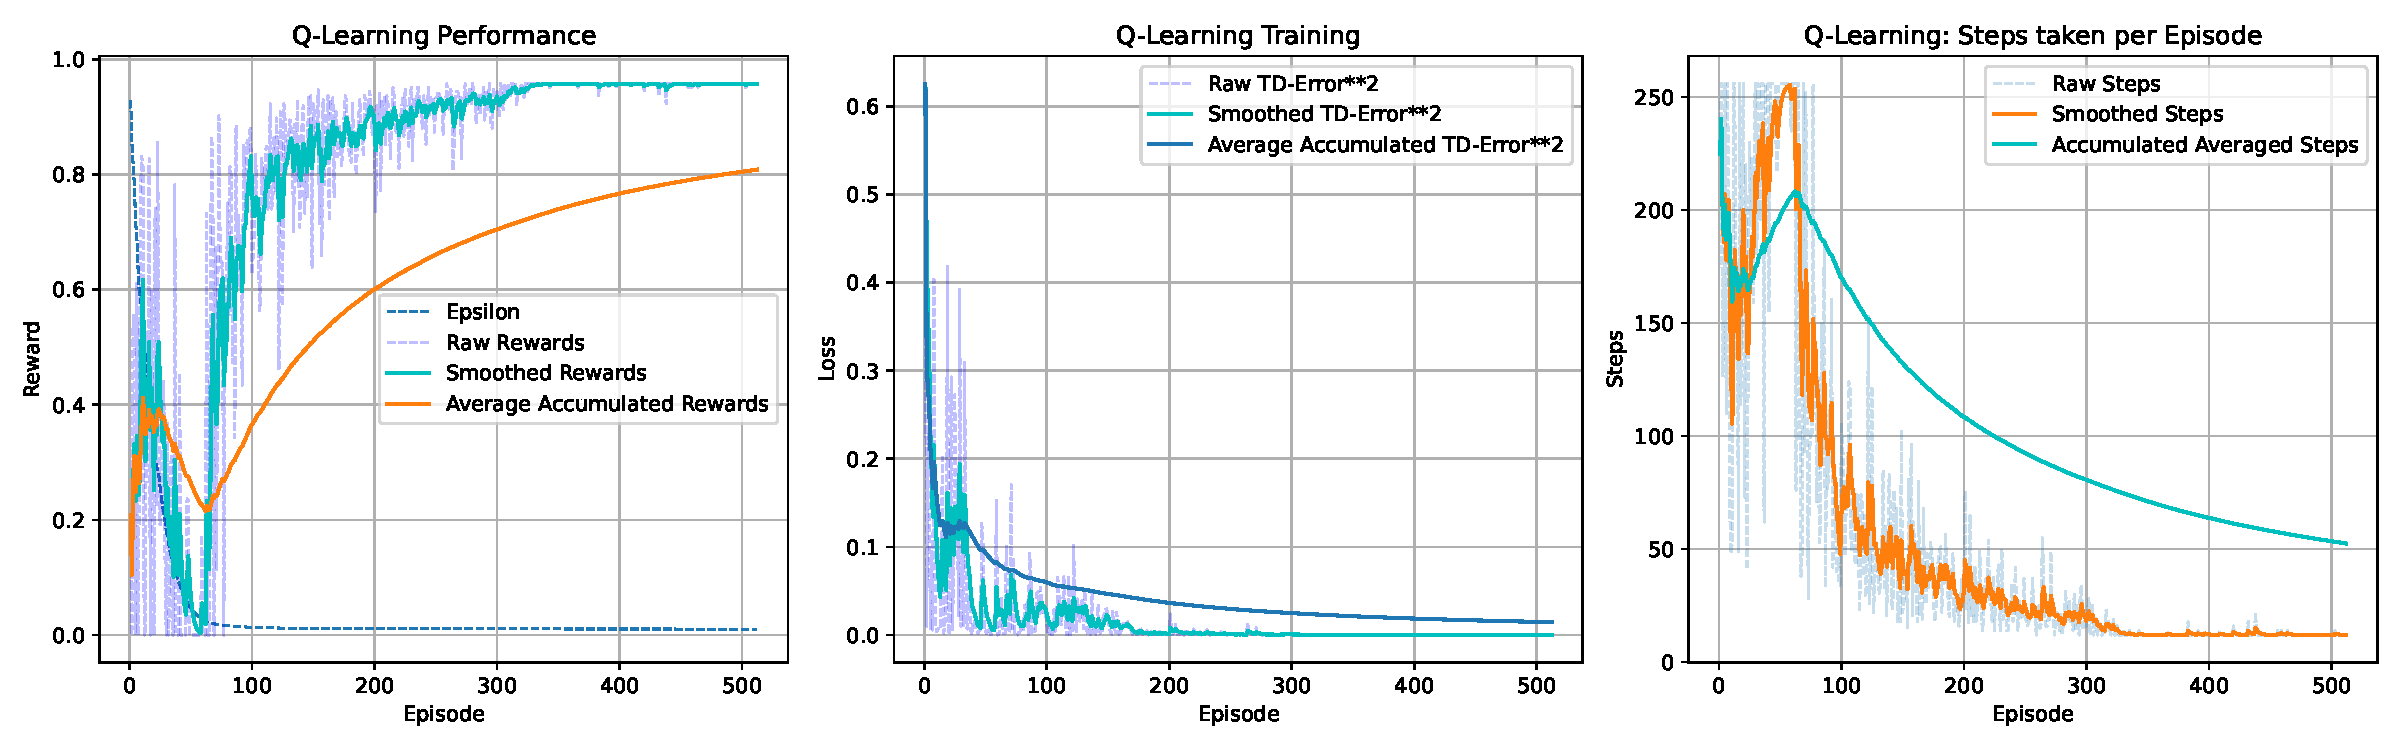
\includegraphics[width=\linewidth]{figures/QLearning_episode.pdf}
	\caption{Q-Learning per episode training metrics}
\end{figure}
\subsection{SARSA-Learning}
\begin{figure}[H]
	\centering
	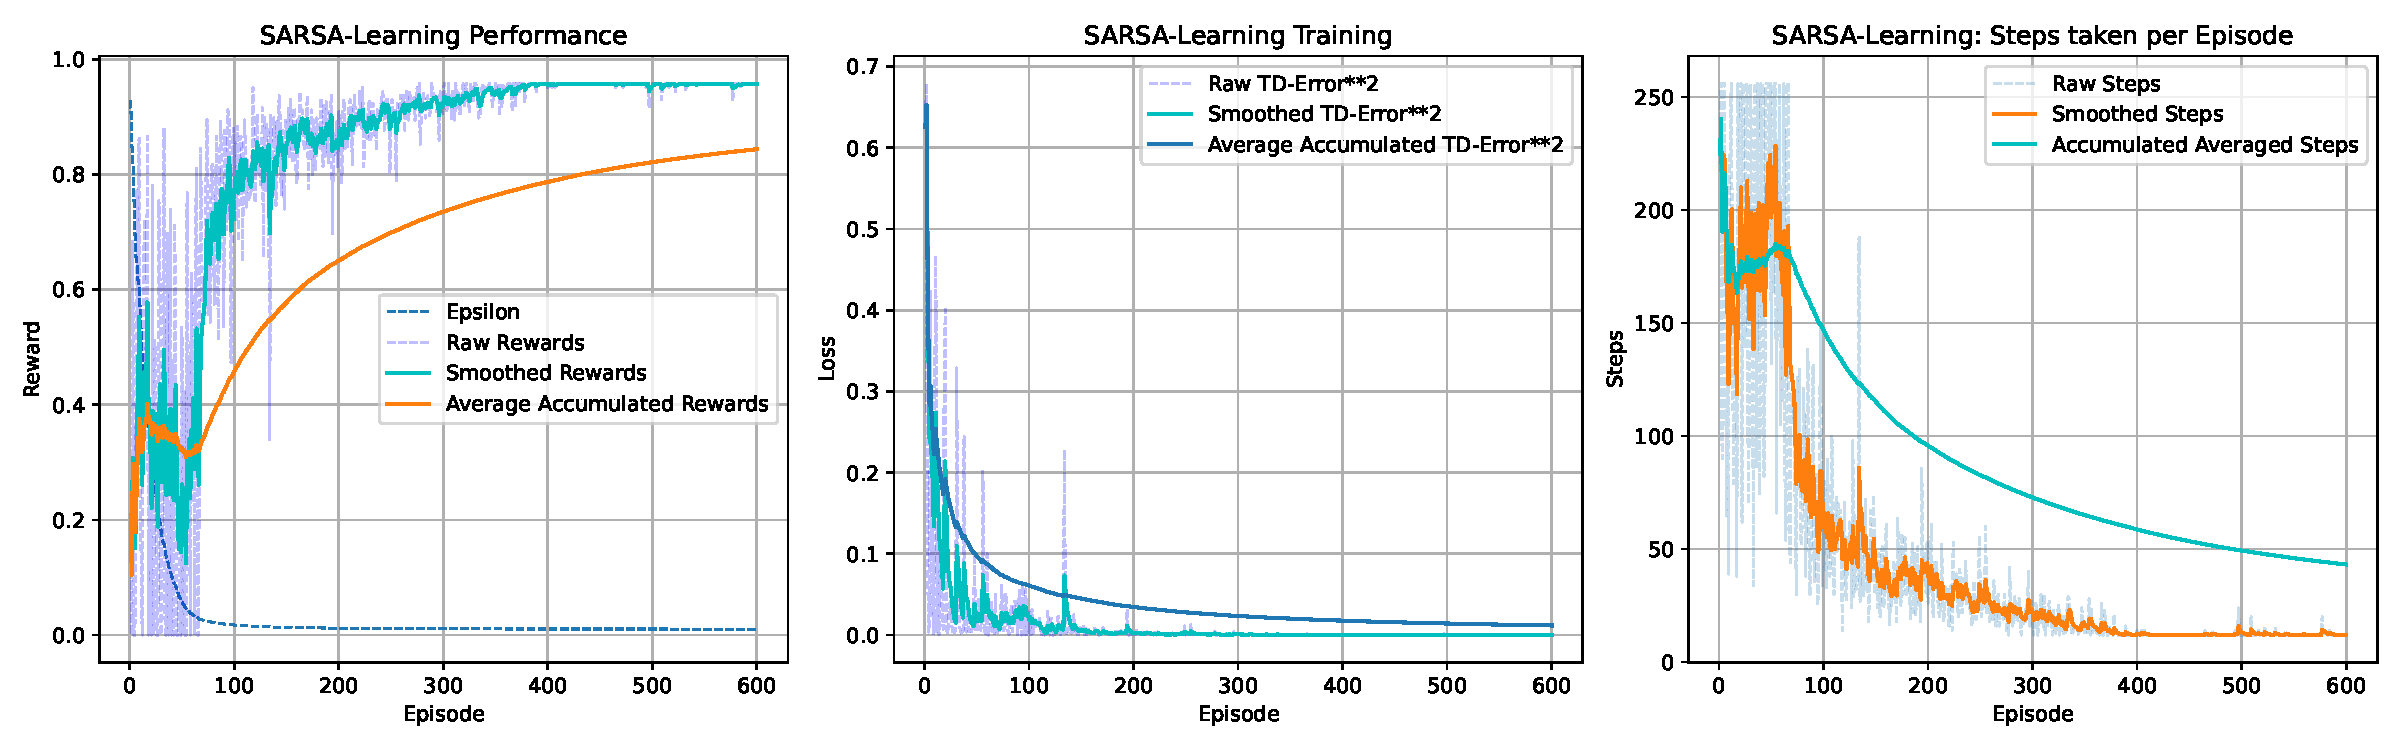
\includegraphics[width=\linewidth]{figures/SARSALearning_episode.pdf}
	\caption{SARSA-Learning per episode training metrics}
\end{figure}
\subsection{Deep Q-Network Learning}
\begin{figure}[H]
	\centering
	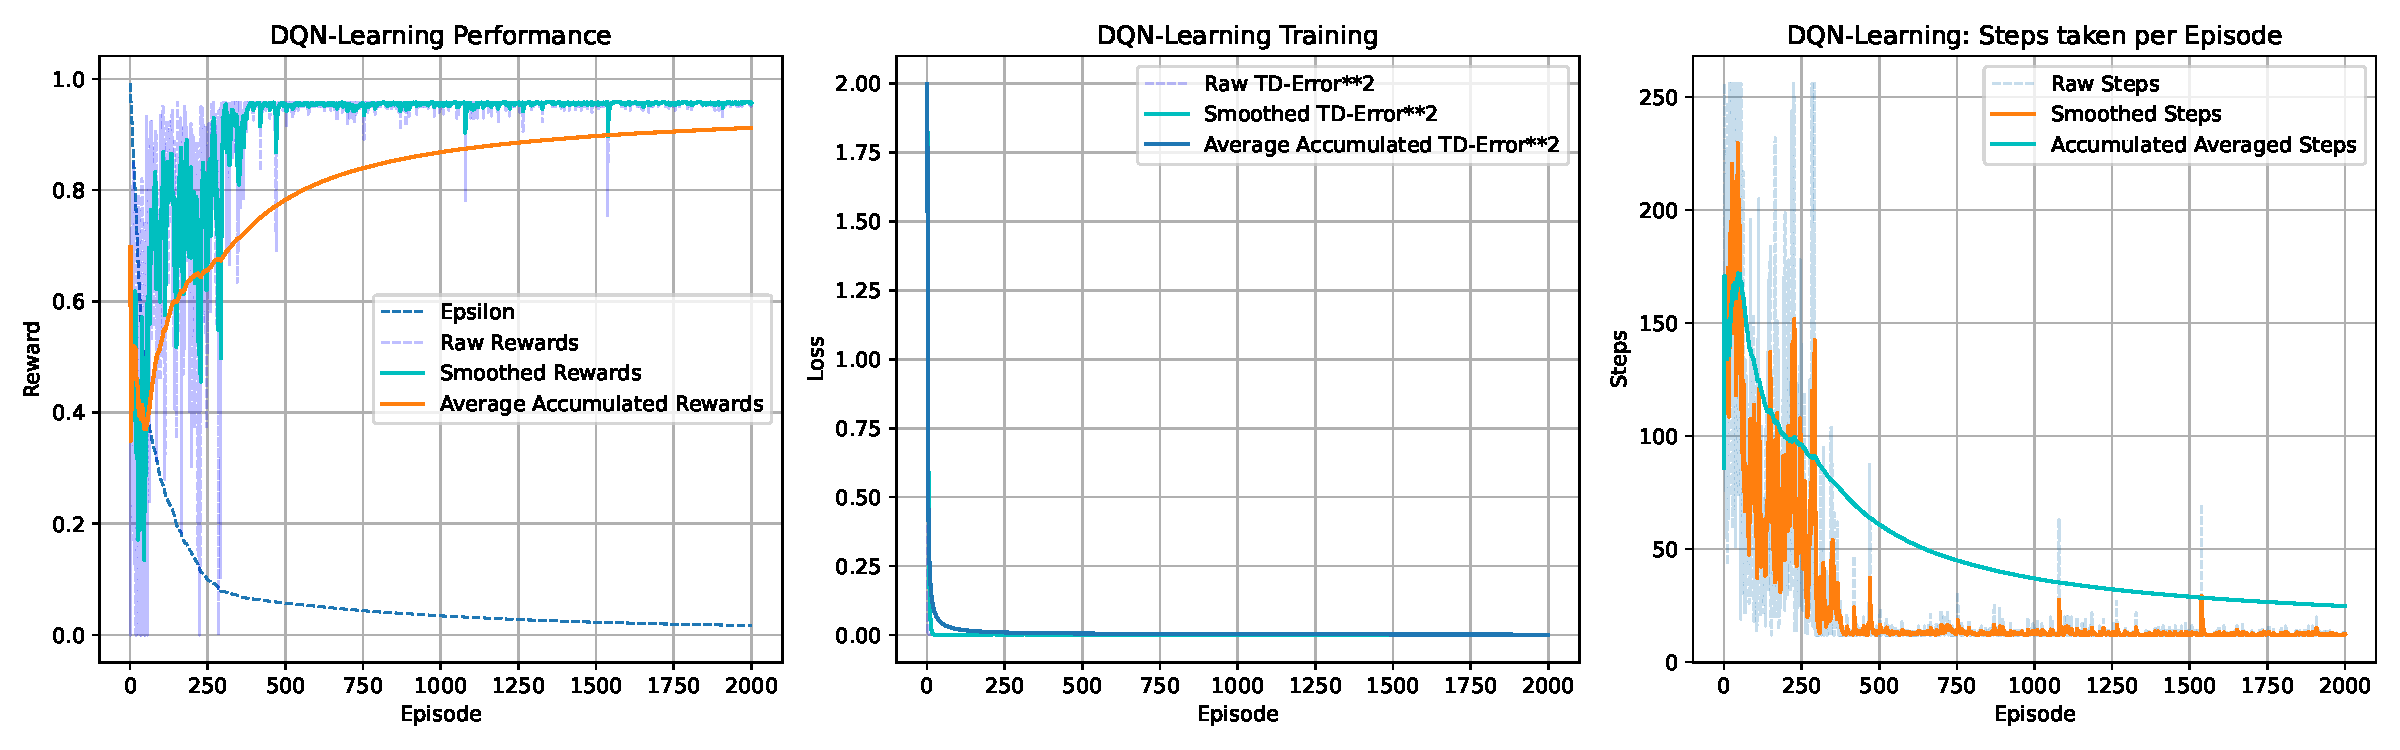
\includegraphics[width=\linewidth]{figures/DQNLearning_episode.pdf}
	\caption{DQN-Learning per episode training metrics}
\end{figure}
\subsection{Deep Q-Network Learning with RGB Image}
\begin{figure}[H]
	\centering
	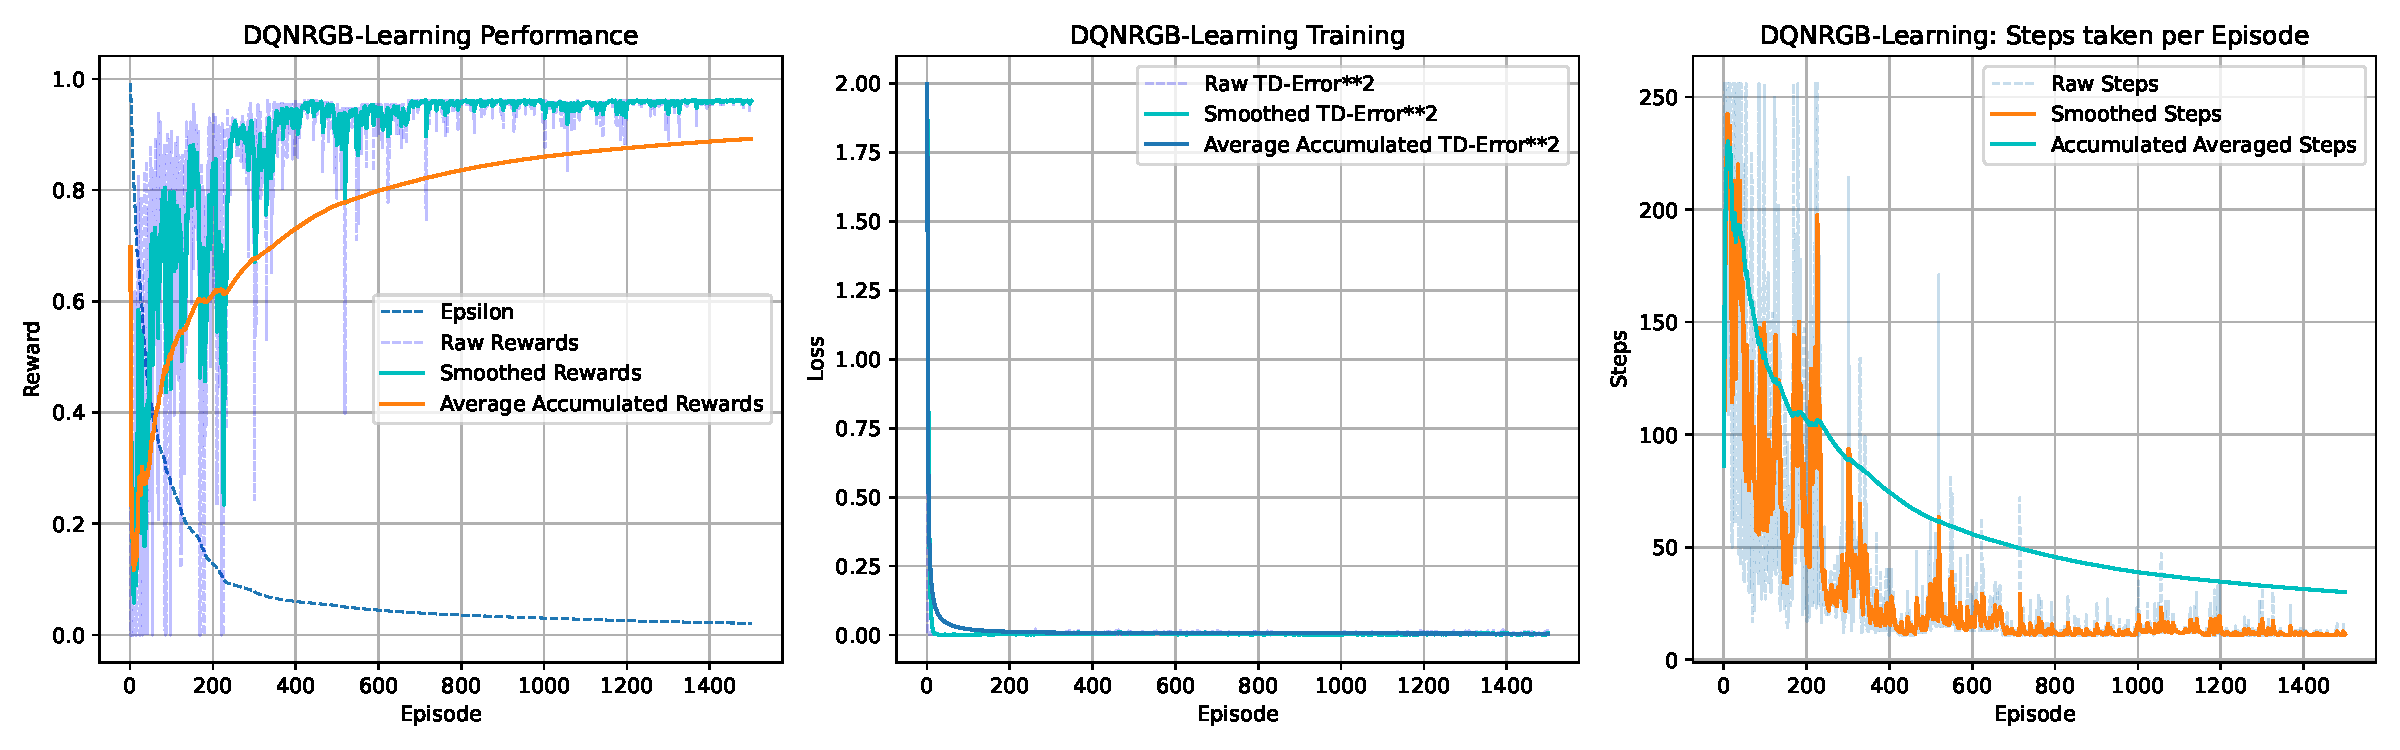
\includegraphics[width=\linewidth]{figures/DQNRGBLearning_episode.pdf}
	\caption{DQN-Learning with RGB Image technique per episode training metrics}
\end{figure}

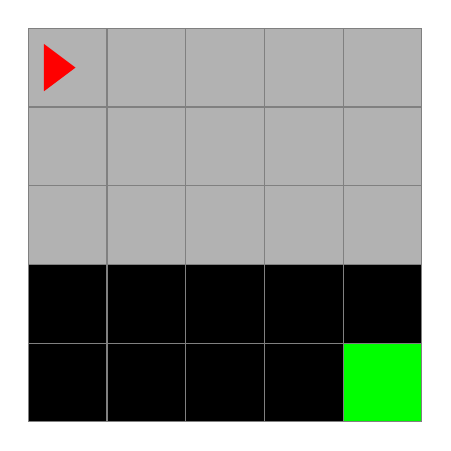
\begin{tikzpicture}

	% Define colors
	\definecolor{darkgray}{rgb}{0.3, 0.3, 0.3}
	\definecolor{lightgray}{rgb}{0.7, 0.7, 0.7}
	\definecolor{green}{rgb}{0, 1, 0}
	\definecolor{red}{rgb}{1, 0, 0}

	% Draw the background
	\fill[darkgray] (0,0) rectangle (5,5);

	% Draw the grid
	\foreach \x in {0, 1, ..., 4} {
		\foreach \y in {2, 3, 4} {
			\fill[lightgray] (\x,\y) rectangle (\x+1,\y+1);
		}
		\foreach \y in {0, 1} {
			\fill[black] (\x,\y) rectangle (\x+1,\y+1);
		}
	}

	% Draw the green square
	\fill[green] (4,0) rectangle (5,1);

	% Draw the red triangle
	\fill[red] (0.2,4.8) -- (0.2,4.2) -- (0.6,4.5) -- cycle;

	% Draw the border lines of the grid
	\foreach \x in {0, 1, 2, 3, 4, 5} {
		\draw[gray] (\x,2) -- (\x,5);
		\draw[gray] (\x,0) -- (\x,2);
	}
	\foreach \y in {0, 1, 2, 3, 4, 5} {
		\draw[gray] (0,\y) -- (5,\y);
	}

\end{tikzpicture}

\section{Conclusion}
%\begin{thebibliography}{1}
%\end{thebibliography}